
\newpage

\thispagestyle{empty}

\noindent

\ifnarrow

\noindent
\begin{tabular}{ @{}p{2.5cm} @{}p{4cm} }

  \begin{minipage}{2.5cm}
    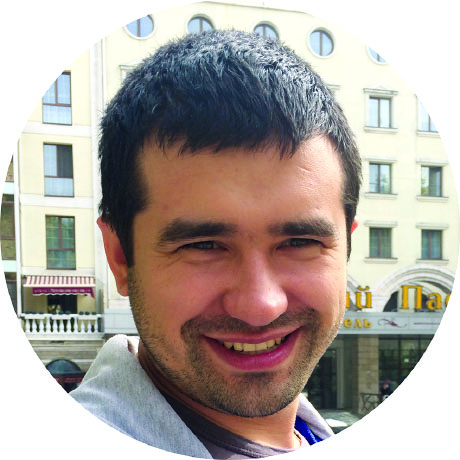
\includegraphics[width=2cm, height=2cm]{media/avatar.jpg}
  \end{minipage}

&
  \vspace{0.25cm}
  {\Large\textbf{Об авторе}}

\end{tabular}
\noindent
Иван Гришаев~--- увлечённый программист. Последние пять лет пишет на
Clojure. Работает удалённо в Exoscale (Швейцария). Специализируется на языках
семейства Лисп и~редакторе Emacs. Сооснователь IT-сообщества <<Глубокий
рефакторинг>> в~Воронеже. Ведёт блог о программировании и удалённой работе
\SITELINK.

\else

\begin{tabular}{ @{}p{2.5cm} @{}p{5cm} }

\begin{minipage}{2.5cm}
  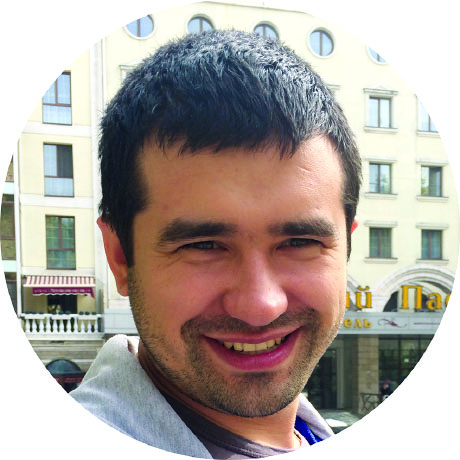
\includegraphics[width=2cm, height=2cm]{media/avatar.jpg}
\end{minipage}

&

\vspace{-1cm}

\section*{Об авторе}

Иван Гришаев~--- увлечённый программист. Последние пять лет пишет на
Clojure. Работает удалённо в Exoscale (Швейцария). Специализируется на языках
семейства Лисп и~редакторе Emacs. Сооснователь IT-сообщества <<Глубокий
рефакторинг>> в~Воронеже. Ведёт блог о программировании и удалённой работе
\SITELINK.

\end{tabular}
\fi
